\documentclass[a4paper,12pt]{article}
\usepackage{float}
\usepackage{hyperref}
\usepackage{graphicx}

\title{Final report}
\author{The Waypointers}

\begin{document}

%%%%%%%%%%%%%%%%%%%%%%%%%%%%%%%%%%%%%%%%%
% University Assignment Title Page
% LaTeX Template
%
% This template has been downloaded from:
% http://www.LaTeXTemplates.com
%
% Original author:
% WikiBooks (http://en.wikibooks.org/wiki/LaTeX/Title_Creation)
%
% License:
% CC BY-NC-SA 3.0 (http://creativecommons.org/licenses/by-nc-sa/3.0/)i

\begin{titlepage}

\newcommand{\HRule}{\rule{\linewidth}{0.5mm}} % Defines a new command for the horizontal lines, change thickness here

\center % Center everything on the page

%----------------------------------------------------------------------------------------
%	HEADING SECTIONS
%----------------------------------------------------------------------------------------

\textsc{\LARGE King's College London}\\[1.5cm] % Name of your university/college
\textsc{\Large 7CCSMGPR Group Project}\\[0.5cm] % Major heading such as course name
%\textsc{\large Minor Heading}\\[0.5cm] % Minor heading such as course title

%----------------------------------------------------------------------------------------
%	TITLE SECTION
%----------------------------------------------------------------------------------------

\HRule \\[0.4cm]
{ \huge \bfseries Final project report}\\[0.4cm] % Title of your document
\HRule \\[1.5cm]

%----------------------------------------------------------------------------------------
%	AUTHOR SECTION
%----------------------------------------------------------------------------------------
\begin{flushleft}
{\Large \emph{Team:}\\
\textsc{The Waypointers}\\}
Haipei Liu\\
Karlo Santini\\
Michal Szewczak\\
Mengzhu Wang\\
Minghao Zhu\\[3cm]
\end{flushleft}
%----------------------------------------------------------------------------------------
%	DATE SECTION
%----------------------------------------------------------------------------------------

{\large \today}\\[3cm] % Date, change the \today to a set date if you want to be precise

%----------------------------------------------------------------------------------------
%	LOGO SECTION
%----------------------------------------------------------------------------------------

%\includegraphics{Logo}\\[1cm] % Include a department/university logo - this will require the graphicx package

%----------------------------------------------------------------------------------------

\vfill % Fill the rest of the page with whitespace

\end{titlepage}

%%%%%%%%%%%%%%%%%%%%%%%%%%%%%%%%%%%%%%%%%%

\tableofcontents

\section{Introduction}

\section{Review of related work}
To make a higher achievement, some research of background and review of existed traffic simulators have been done before the start of the design and programming.\\
\subsection{Background}
Traffic simulation system is a model of transportation systems by employing the application of computer software to analyse the whole traffic of a city and help plan, design and operate transportation systems.\\
Over forty years ago, the systems of transportation simulation started. By nowadays, it has been a vital area of discipline in traffic engineering and transportation planning. Various nations are using simulation to aid in their management of transportation networks and different academic institutions are working on the development of the traffic simulation system.\\
This kind of Simulation can study models too complicated for analytical or numerical treatment, can be used for experimental studies, can study detailed relations that might be lost in analytical or numerical treatment and can produce attractive visual demonstrations of present and future scenarios.\\
For the application of traffic simulation, the models are useful from different perspectives. Simulation can be applied to both transportation planning and to traffic system design and operations. In the planning, the simulation models evaluate the impacts of regional urban development patterns on the performance of the transportation infrastructure. Some organizations who works on regional planning use these models to evaluate what-if scenarios in the region. On another side, modeling of transportation system can focus on the operations and design of a smaller scale such as lane types, traffic lights timing and some other related questions. They are investigated to improve local system effectiveness and efficiency.\\
The traffic simulation system can be used for various types of transportation modes whether it is for operations or planning.\\
Traffic simulation software is getting better in different ways. With new achievements in computing, mathematics and engineering, simulation software programs are becoming much more powerful, faster, more realistic and more detail oriented.\\
In general, transportation models can be classified into different models: macroscopic, mesoscopic, and microscopic. Macroscopic models analyse aggregated characteristics of transportation elements, for example, aggregated traffic flow dynamics and zonal-level travel demand analysis. Mesoscopic models deal with traffic elements in small groups, within homogeneously considered elements, such as vehicle platoon dynamics and household-level travel behaviour. Microscopic models focus on individual elements of transportation systems, such as individual vehicle dynamics.
After learning of the background, some of the existed traffic simulators will be discussed in next section.\\
\subsection{Existed traffic simulation software}
By searching online, plenty of existed software with different functions can be found.\\
\subsubsection{Traffic-Simulation.de html5 Version: Ring Road}
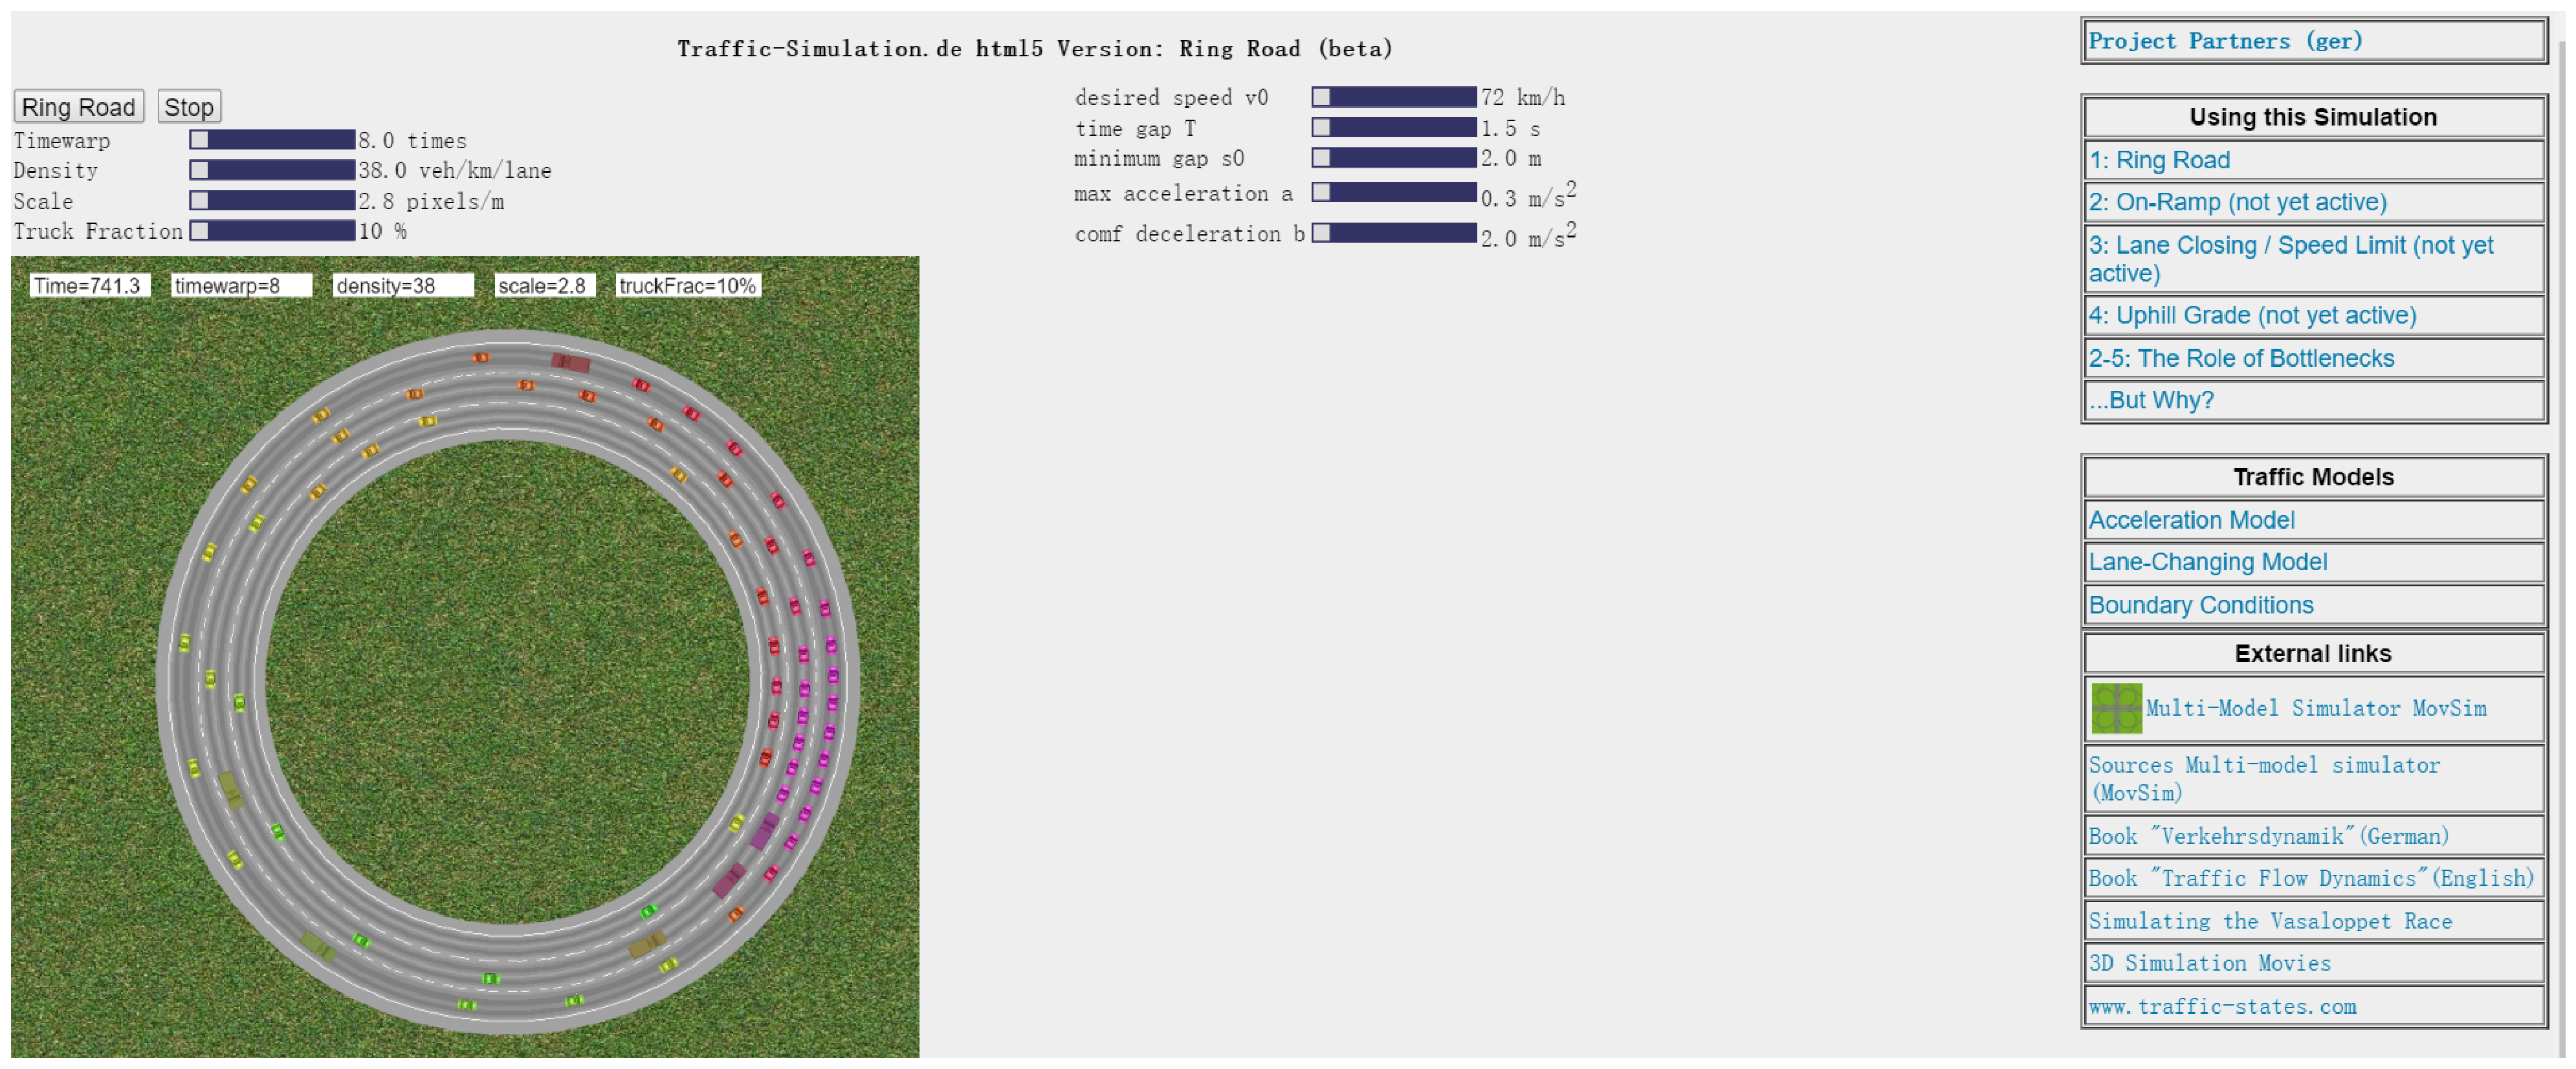
\includegraphics[width=12.5cm]{RingRoad.eps}\\
As shown in the figure, this simulator is literally a web page programmed in HTML (Hypertext Markup Language) which mainly used to test the traffic jams and congestion of a Ring Road with various parameters.\\
There are 2 parameters about ‘time’. The first one is ‘Timewarp’ and another is ‘time gap’.\\
Timewarp is related to the changing speed of the whole system. In another word, it is the time of all the vehicles. By changing it, the relative velocity between vehicles will be constant.\\
On the contrary, the time-gap is the changing of the relative velocity between vehicles.\\
The parameter ‘Density’ is the number of vehicles in one map and the parameter ‘Scale’ is used to enable the user to change the size of the simulator. The ‘Truck Fraction’ will control the number of trucks, the ‘desired speed’ is the speed that all the vehicles would like to achieve and the ‘minimum gap’ is the minimum distance between vehicles.\\
Also, this traffic simulation system provides different traffic models for users to analyse. By changing the parameters, the condition of the traffic jam and congestion can be recognized in real time easily.\\
\subsubsection{RoadTrafficSimulator}
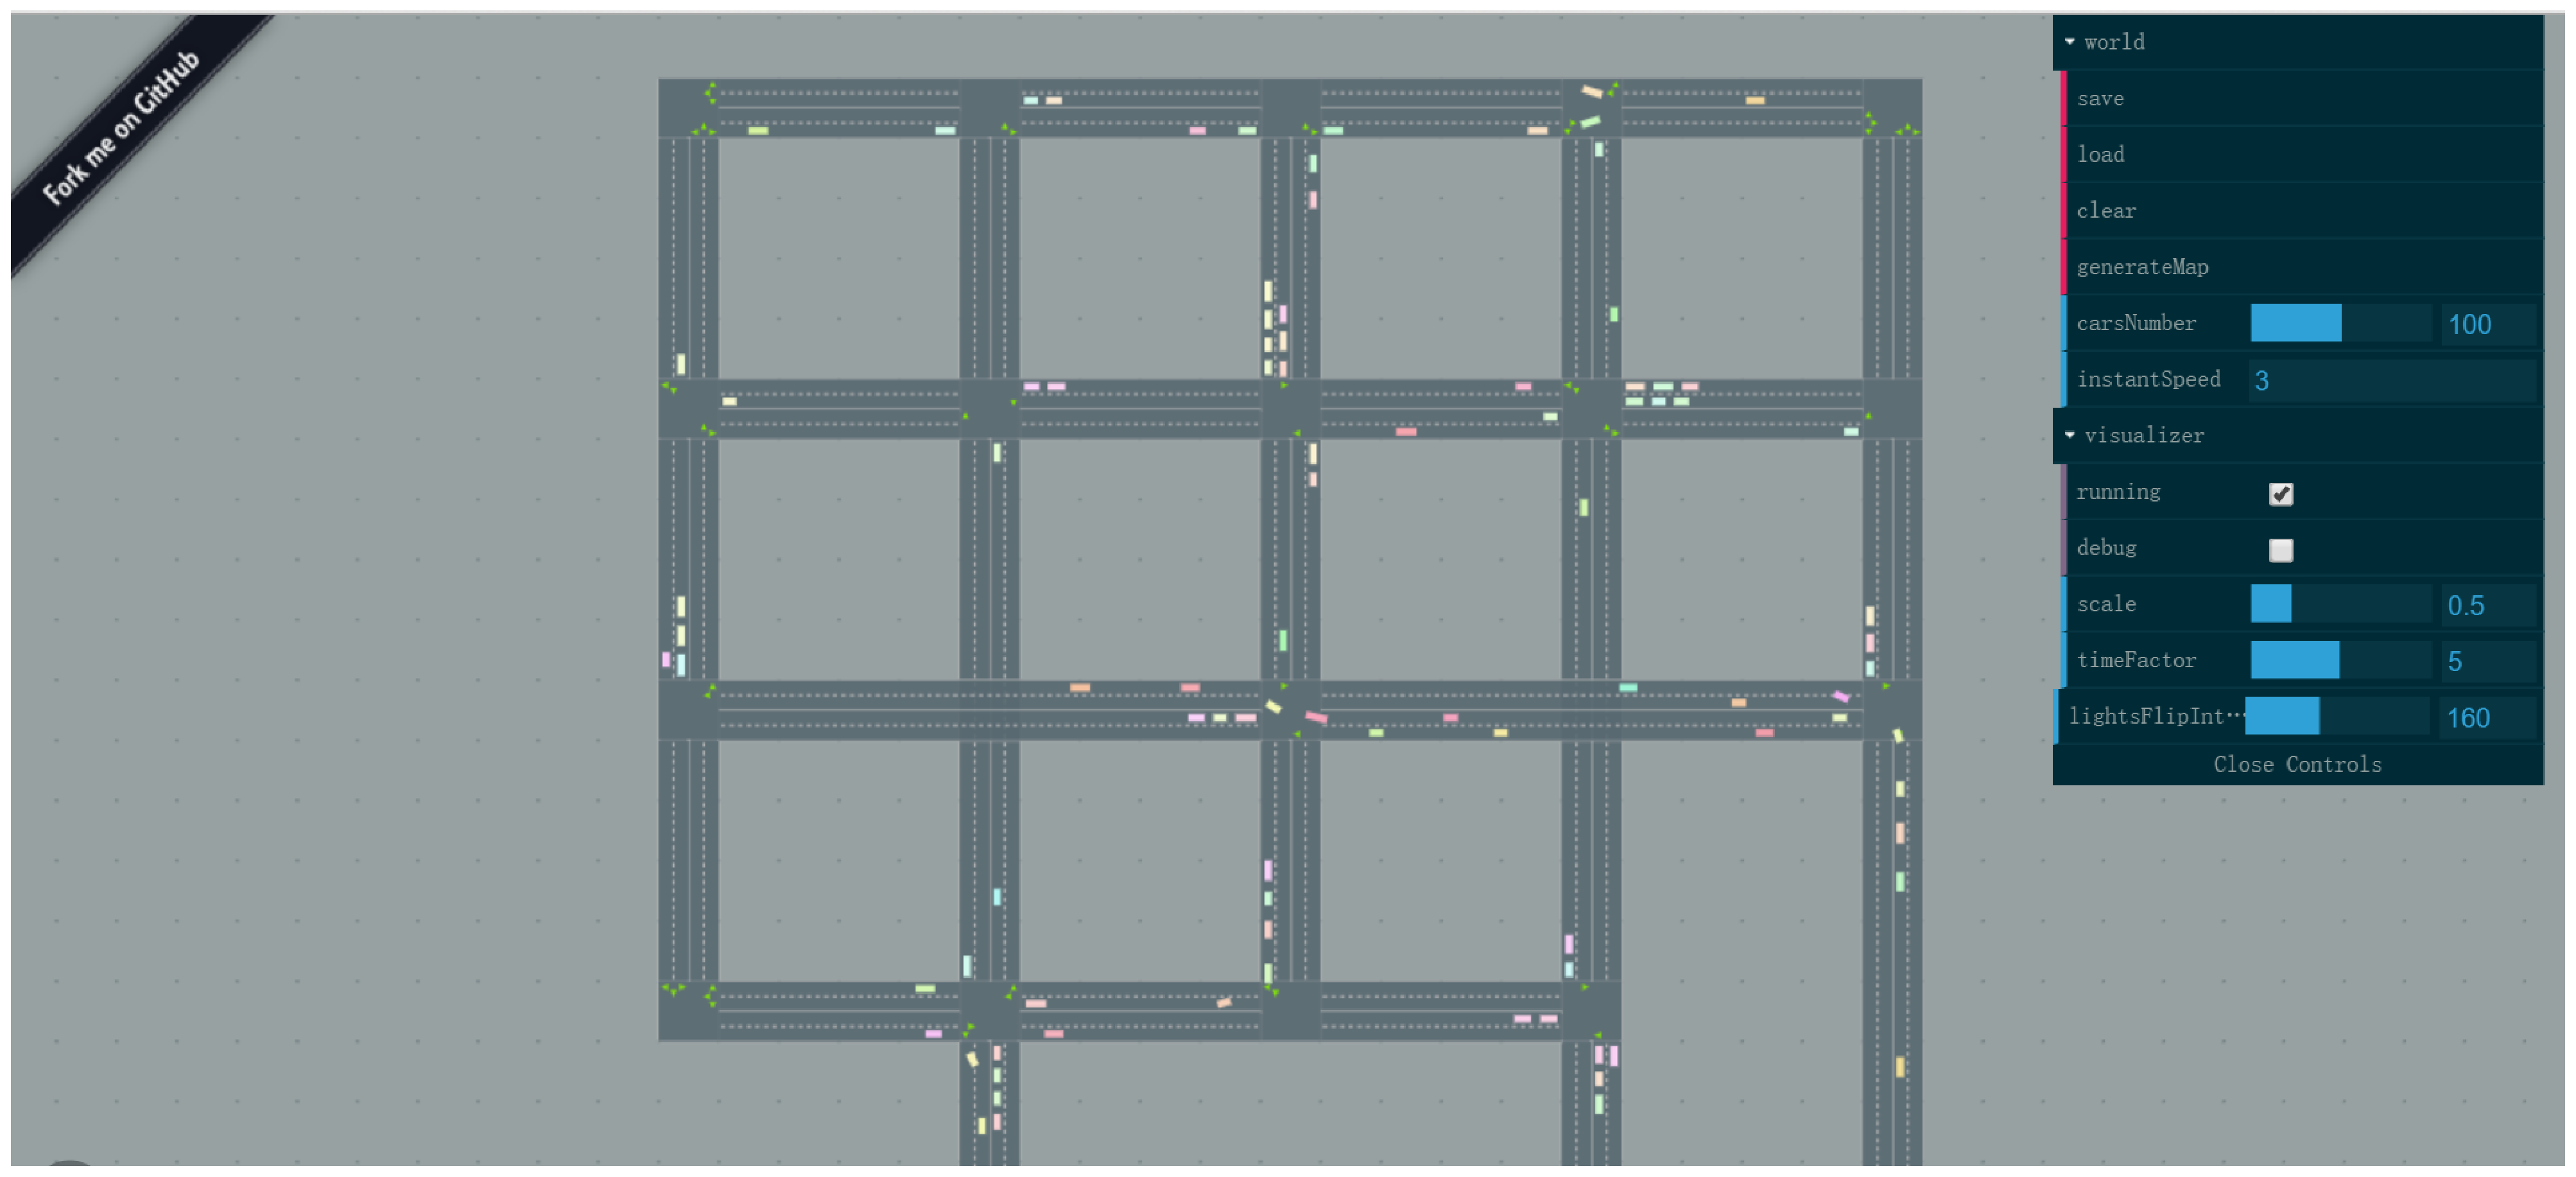
\includegraphics[width=12.5cm]{RoadTrafficSimulator.eps}\\
This road traffic simulator is more similar to a road map in the real world. This system is also made by HTML but the main usage of the simulator differs from the ring road traffic simulation. As a road traffic simulator, this system contains roads, junctions, traffic lights and different types of vehicles.
As is demonstrated in the figure, each road has two directions and each direction has two lanes. In this case, the vehicles are able to change lane. Similarly, there are also some parameters in the simulator for users to change.\\
There are 2 highlights in this simulator. Firstly, it enables users to generate the map randomly which is allowed to try different maps to test the traffic system and makes the simulator more reliable. Secondly, the gap of traffic light time changing can be altered. Users can find the best time changing of the traffic light and get the best demonstration of the road simulation.\\
By studying and analysing the background and the existed traffic simulation system. The group members discussed the aim functions and the main requirements and design. In the next section, the details can be discussed. The programming language employed is Java.\\

\section{Requirements}

\section{Design}

\section{Implementation}
\subsection{Test}
After finishing the programming of the functions. ‘Test’ is a significant part of the whole project. However, it is too complex to test the units manually. Also, it is not able to find the exact location of the BUGs in the programme.\\
In this case, it is crucial to create a test class to check if the units work well.\\
\subsubsection{JUnit}
JUnit is a unit testing framework for the Java programming language.It has been a significant part in the development of test-driven development and is one of a family of unit testing frameworks which is collectively known as xUnit that originated with SUnit.\\
In 2013, there is a research survey hosted on GitHub across 10,000 Java projects performed found that JUnit was the most popular and commonly used  included external library. Each library was used by 30.7 percent of projects.\\
JUnit provides overloaded assertion methods for all primitive types and Objects and arrays (of primitives or Objects). In this method, the parameter order is expected value followed by actual value. Optionally the first parameter can be a String message that is output on failure. There is a slightly different assertion, assertThat that has parameters of the optional failure message, the actual value, and a Matcher object. It needs to be notice that expected and actual are reversed compared to the other assert methods.\\
In this project, 3 main motheds are utilized: ‘arrange’ ‘act’ and ‘assert’ and the most important method is assertThat.\\
\subsubsection{What tested}
There are two main class tested in this project. MapDTO and MapWorldStateFactory.\\
The main aim to test the MapDTO is to check if this class can generate the map properly.In the test of MapDTO, different number of roads are added in the ‘act’ mothed and in the ‘assert’ the number of junctions, number of nodes ,number of roads and the road direction are checked to test if the map are generated correctly.\\
Beside, MapWorldStateFactory helps convert existed ‘xml’ format maps to the maps will be shown in GUI. By testing this class, it is able to know if both MapWorldStateFactory and RoadMap class works well because the MapWorldStateFactory go through to RoadMap.\\
The functions tested are the junctions, number of junctions, number of nodes, number of roads and the direction of roads and the details of traffic lights.\\
After testing, BUGs are found and fixed by debuging.\\
\section{Teamwork}

\subsection{Tools and libraries used}

\subsubsection*{Tools and applications}

\begin{itemize}
	\item Git\footnote{\url{https://git-scm.com/}} - version control
	\item GitHub\footnote{\url{https://github.com/}} - Git repository management, task assignment, teamwork
	\item \LaTeX\footnote{\url{https://www.latex-project.org/}} - typesetting system, for creating documentation
	\item Gliffy\footnote{\url{https://www.gliffy.com/}} - a Chrome app for creating diagrams
	\item Apache Maven\footnote{\url{https://maven.apache.org/}} - a build tool for building the project easily and for dependency management
	\item Travis CI\footnote{\url{https://travis-ci.org/}} - a continuous integration tool that integrates into GitHub and builds every commit pushed to the repository (in our case - using Maven), also checking if the tests pass
	\item IntelliJ IDEA\footnote{\url{https://www.jetbrains.com/idea/}} - a cross-platform IDE for development in Java (and more). To minimize potential hassles with different development environments, we all agreed on using the same IDE.
\end{itemize}


A significant fact to note that is our team used all the major operating systems (Windows, OS X, Linux), so we focused on choosing cross-platform tools. The only troubles that arised from that were minor layout differences in the Swing GUI of our system.

\subsubsection*{Libraries}

\begin{itemize}
	\item JDK 1.8\footnote{\url{http://www.oracle.com/technetwork/java/javase/downloads/index.html}} - We had several reasons for choosing Java: \begin{itemize}
		\item Familiarity of team members with it
		\item Available on all platforms
		\item Good capabilities of cross-platform GUI
		\item Strong typing allowing for easier maintaining of code integrity
	\end{itemize}
	We chose version 8 because it introduces many much-needed improvements for the language like lambda functions or the Stream API.
	\item JUnit 4.12\footnote{\url{http://junit.org/junit4/}} - The ``de facto'' unit testing library for Java. Good integration with IntelliJ IDEA and Maven.
	\item FEST-Assert 2.0M5\footnote{\url{https://github.com/alexruiz/fest-assert-2.x}} - A library to make assertions in unit tests more readable and easier to compose.
	\item JGraphT 0.7.3 \footnote{\url{http://jgrapht.org/}} - A graph library to take advantage of graph representation of the road network, mainly pathfinding for vehicles.
	\item XStream 1.2.2 \footnote{\url{http://x-stream.github.io/}} - An XML serialization library to bring reading and writing XML road maps to life.
\end{itemize}



\section{Evaluation}

\section{Peer assessment}

\end{document}